\documentclass[UTF8]{ctexart}
\usepackage{graphicx}
\usepackage{booktabs}
\usepackage{amsmath}
\usepackage{caption}
\usepackage{subcaption}
\usepackage{lmodern}
\usepackage{float}
\usepackage{geometry}
\geometry{margin=1in}

\usepackage{listings} % 添加这一行

\title{分布式能源实践作业报告}
\author{姓名:唐玮嘉 \\ 学号:2023428020130 \\ 班级:23能动一班(化能杨班)}
\date{\today}

\begin{document}

\maketitle

\begin{abstract}
本报告围绕分布式能源在宾馆场景下的应用展开,通过对宾馆月平均热电比、各季总负荷逐时折线图、各季逐时折线图以及月平均能耗消费结构的分析,旨在深入了解宾馆能源消耗的特性和规律,为分布式能源系统的优化提供依据。
\end{abstract}

\section{引言}
随着能源问题的日益突出,分布式能源系统在宾馆等建筑中的应用越来越受到关注。对宾馆能源消耗情况进行深入分析,有助于合理规划能源供应,提高能源利用效率,降低运营成本。本实践通过对宾馆相关能源数据的处理和可视化,旨在揭示能源消耗的内在规律。

\section{研究方法}
本研究主要采用数据收集、处理和可视化的方法。首先,收集宾馆的能源消耗数据,包括电力、热力等方面的信息。然后,使用 Python 编程语言对数据进行处理和分析,计算月平均热电比、各季总负荷和逐时负荷等指标。最后,利用绘图工具绘制相应的图表,直观展示能源消耗的情况。

\section{结果与分析}

\subsection{宾馆月平均热电比}
月平均热电比是衡量宾馆能源利用效率的重要指标。通过计算每个月的热电比并取平均值,可以得到宾馆月平均热电比的变化趋势。

为了计算月平均热电比,我们首先从数据中提取每月的热负荷和电负荷数据。热负荷数据反映了宾馆在加热、热水供应等方面的能源需求,而电负荷数据则体现了宾馆在照明、电器设备运行等方面的电力消耗。然后,将每月的热负荷除以电负荷,得到每月的热电比。最后,对每个月的热电比进行平均,得到月平均热电比。

图 \ref{fig:monthly_thermoelectric_ratio} 展示了宾馆月平均热电比的变化情况。从图中可以看出,热电比在不同月份存在一定的波动。这可能与季节变化、宾馆的运营模式等因素有关。例如,在冬季,由于供暖需求增加,热负荷相对较高,热电比可能会偏大;而在夏季,空调等电器设备的使用导致电负荷增加,热电比可能会偏小。

\begin{figure}[H]
    \centering
    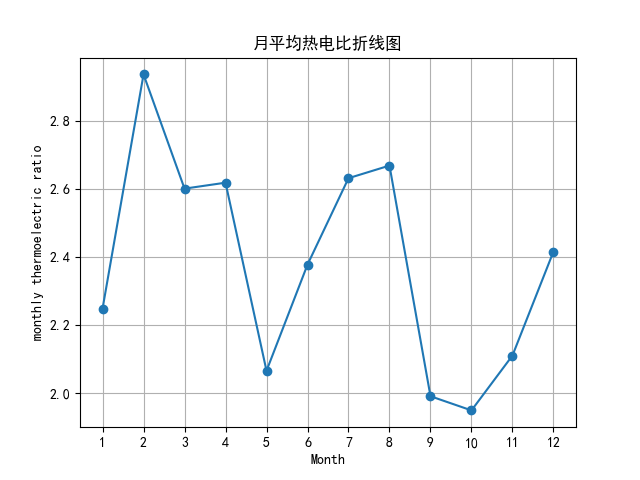
\includegraphics[width=0.8\textwidth]{image/Figure_1.png}
    \caption{宾馆月平均热电比}
    \label{fig:monthly_thermoelectric_ratio}
\end{figure}

\subsection{宾馆各季总负荷逐时折线图}
各季总负荷逐时折线图能够直观地展示宾馆在不同季节的总能源负荷随时间的变化情况。

我们将一年分为夏、冬、过渡季,分别统计每个季节中每天不同时刻的总负荷数据。总负荷包括热负荷和电负荷之和。通过绘制逐时折线图,可以清晰地看到每个季节中总负荷的高峰和低谷时段。

图 \ref{fig:seasonal_total_load} 展示了宾馆各季总负荷逐时折线图。从图中可以看出,不同季节的总负荷曲线具有明显的差异。夏季由于空调的大量使用,总负荷在白天时段较高;而冬季则因为供暖需求,总负荷在夜间和清晨也维持在较高水平。这些信息对于合理安排能源供应,如调整发电设备的运行时间和功率,具有重要的指导意义。

\begin{figure}[H]
    \centering
    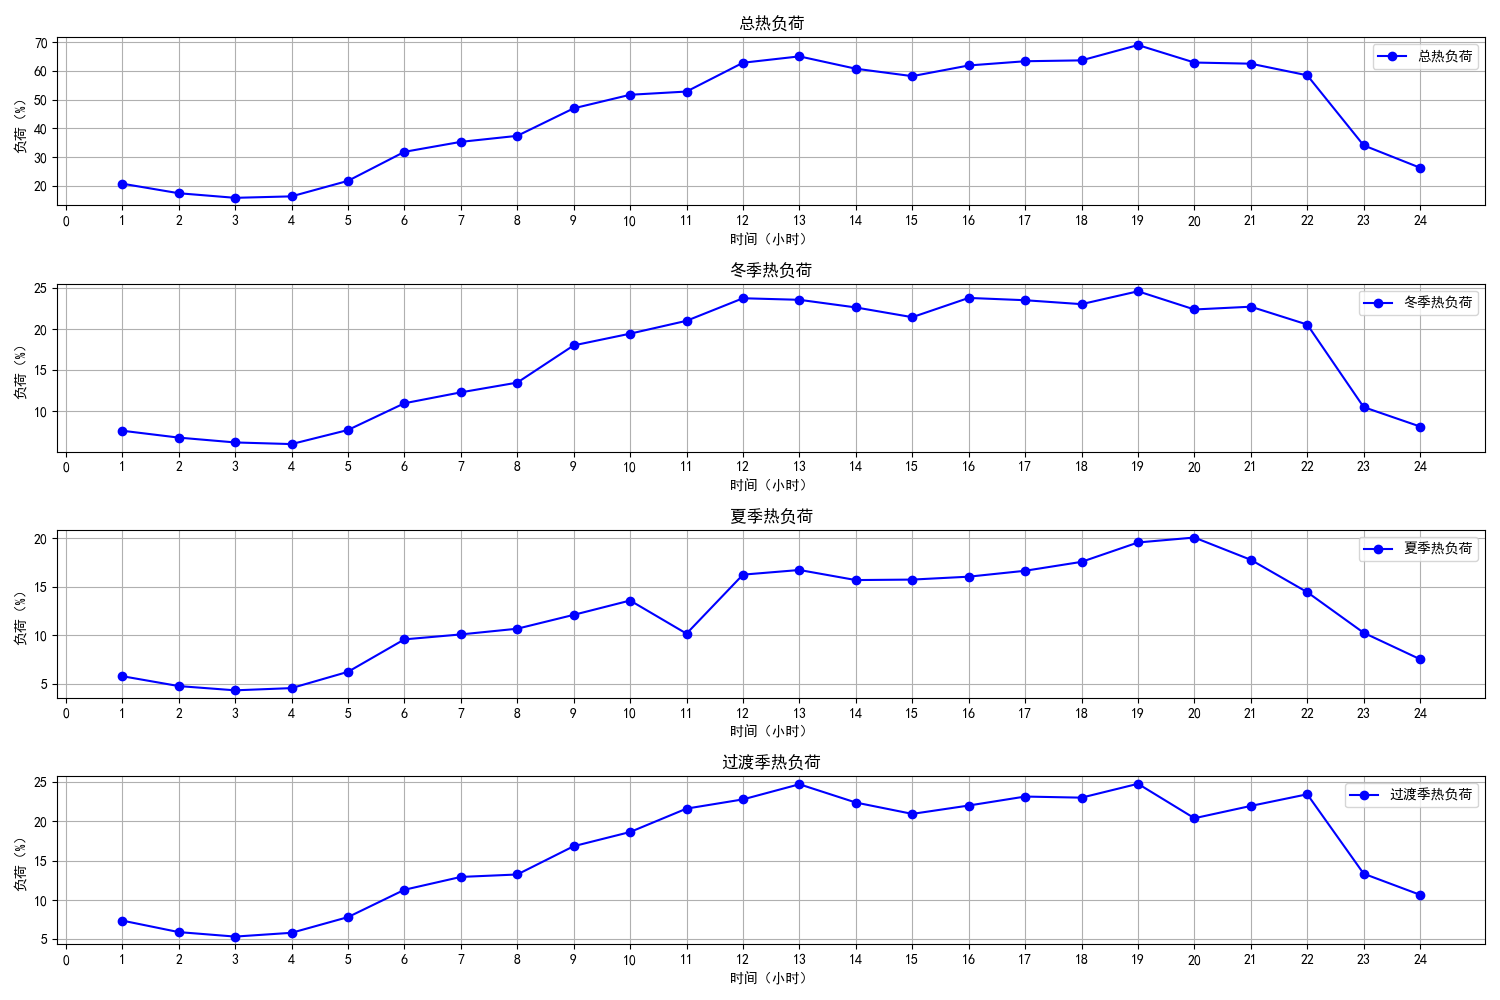
\includegraphics[width=0.8\textwidth]{image/Figure_2.png}
    \caption{宾馆各季总负荷逐时折线图}
    \label{fig:seasonal_total_load}
\end{figure}

\subsection{宾馆各季逐时折线图}
宾馆各季逐时折线图进一步细分了各季节中热负荷和电负荷随时间的变化情况。

同样按照夏、冬、过渡季进行划分,分别绘制每个季节中热负荷和电负荷的逐时折线图。通过对比热负荷和电负荷的曲线,可以更深入地了解宾馆在不同季节的能源消耗特点。

图 \ref{fig:seasonal_hourly_load} 展示了宾馆各季逐时折线图。从图中可以看出,在夏季,电负荷的高峰时段与空调使用的高峰时段相对应,而热负荷相对较低;在冬季,热负荷的高峰时段与供暖需求的高峰时段一致,电负荷也会因为照明、电器设备等的使用而维持在一定水平。这有助于我们根据不同季节的能源需求特点,优化能源分配方案。

\begin{figure}[H]
    \centering
    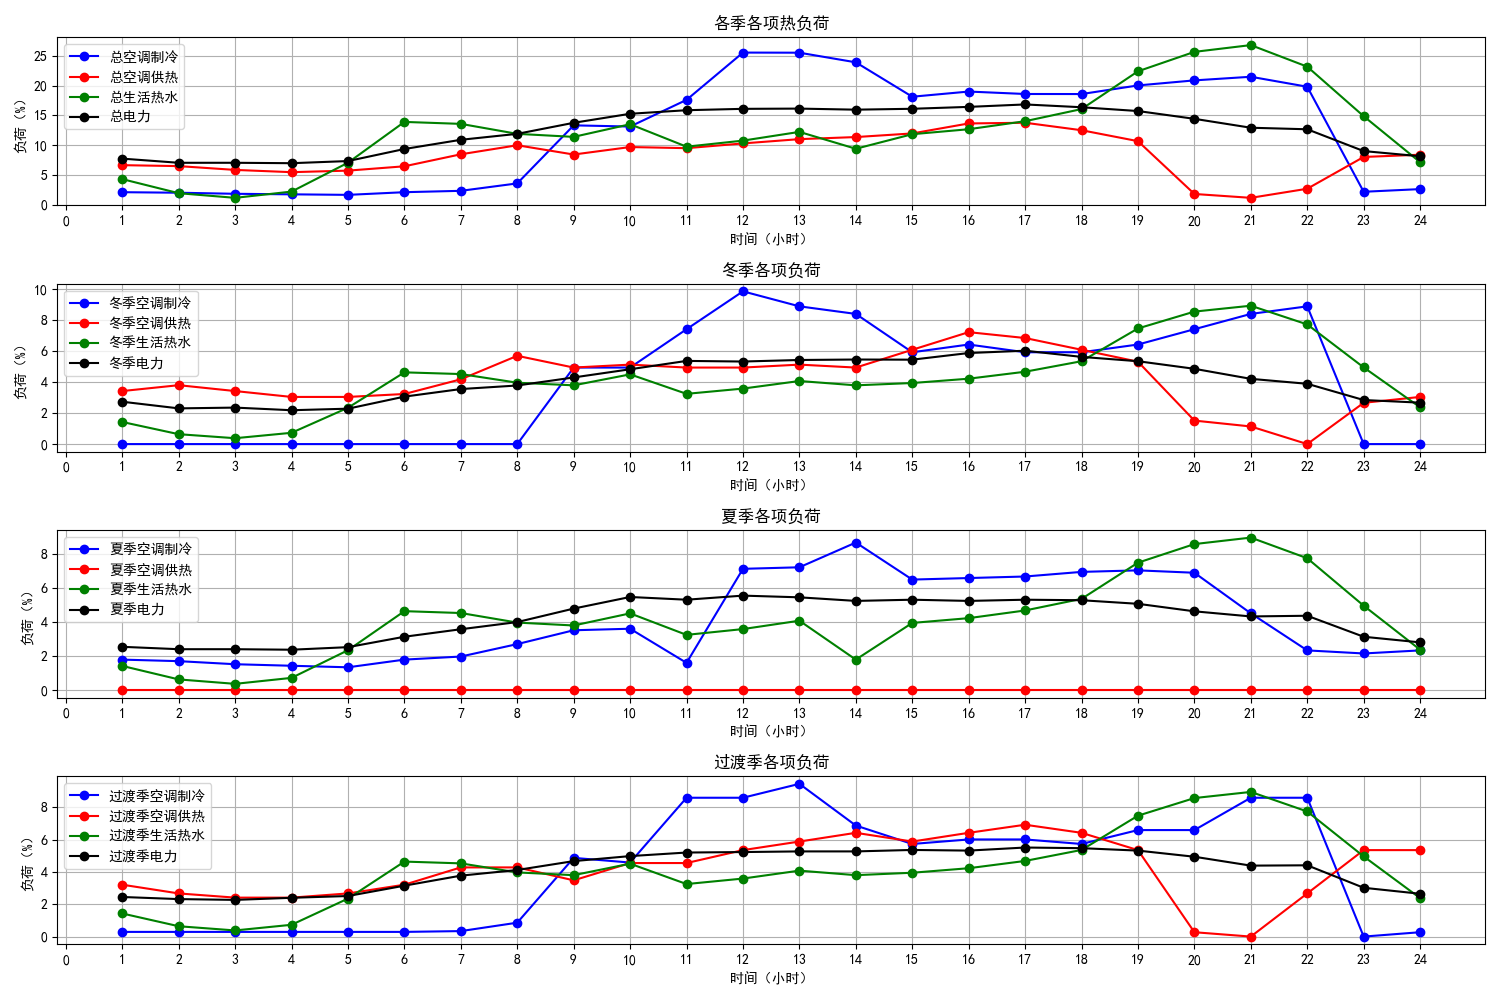
\includegraphics[width=0.8\textwidth]{image/Figure_3.png}
    \caption{宾馆各季逐时折线图}
    \label{fig:seasonal_hourly_load}
\end{figure}

\subsection{宾馆月平均能耗消费结构}
宾馆月平均能耗消费结构反映了宾馆在不同能源类型上的消费比例。

我们统计了宾馆每月在电力、热力等能源类型上的消耗数据,并计算出每种能源类型在总能耗中的占比。通过绘制月平均能耗消费结构图,可以直观地看到宾馆能源消费的结构特点。

图 \ref{fig:monthly_energy_consumption_structure} 展示了宾馆月平均能耗消费结构。从图中可以看出,电力和热力是宾馆主要的能源消耗类型。不同月份的能耗消费结构可能会有所变化,这与季节变化、宾馆的运营活动等因素有关。例如,在冬季,热力的消费占比可能会增加;而在夏季,电力的消费占比可能会提高。了解宾馆月平均能耗消费结构,有助于我们制定针对性的能源管理策略,如优化能源采购、提高能源利用效率等。

\begin{figure}[H]
    \centering
    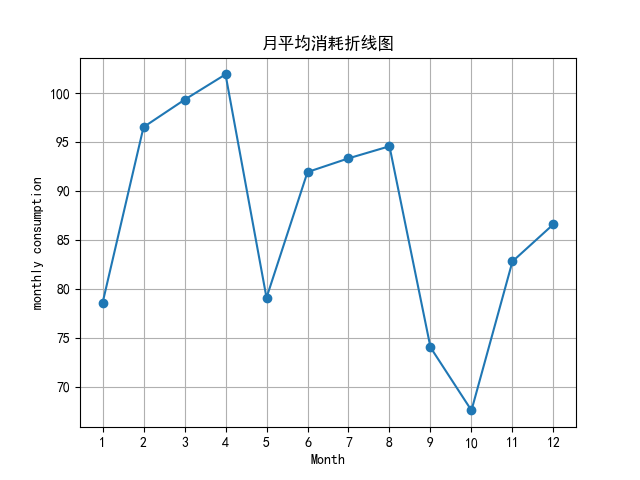
\includegraphics[width=0.8\textwidth]{image/Figure_4.png}
    \caption{宾馆月平均能耗消费结构}
    \label{fig:monthly_energy_consumption_structure}
\end{figure}

\section{结论}
通过对宾馆月平均热电比、各季总负荷逐时折线图、各季逐时折线图以及月平均能耗消费结构的分析,我们得到以下结论:
1. 宾馆月平均热电比存在季节性波动,与季节变化和宾馆运营模式密切相关。
2. 各季总负荷逐时折线图和各季逐时折线图清晰地展示了不同季节的能源负荷特点,为能源供应的合理安排提供了依据。
3. 宾馆月平均能耗消费结构表明电力和热力是主要的能源消耗类型,且不同月份的消费结构有所变化。

基于以上结论,我们建议在宾馆的能源管理中,根据季节变化和能源负荷特点,合理调整能源供应方案,优化能源采购策略,提高能源利用效率,以降低能源成本,实现可持续发展。

\section{附录}
%%代码

%%第一个代码,月平均热电比
\begin{lstlisting}[language=Python]
    import pandas as pd
    import matplotlib.pyplot as plt
    
    # 设置支持中文的字体
    plt.rcParams['font.sans-serif'] = ['SimHei']  # 使用黑体字体
    # 解决负号显示问题
    plt.rcParams['axes.unicode_minus'] = False  
    
    # 读取Excel文件
    df = pd.read_excel("month.xlsx")   
    
    # 筛选出月份列中不是全年的数据
    df = df[df['月份'] != '全年']
    
    # 将月份列转换为整数类型
    df['月份'] = df['月份'].astype(int)
    
    # 计算月平均热电比,热电比 = (空调制冷 + 空调供热 + 生活热水 ) / 电力
    monthly_thermoelectric_ratio = (df['空调制冷'] + df['空调供热'] + df['生活热水']) / df['电力']
    
    
    # 绘制月平均热电比折线图
    plt.plot(df['月份'], monthly_thermoelectric_ratio, marker='o')
    plt.xlabel('Month')
    plt.ylabel('monthly thermoelectric ratio')
    plt.title('月平均热电比折线图')
    plt.grid(True)
    plt.xticks(df['月份']) # 添加x轴刻度标签
    plt.show()
    
\end{lstlisting}

%%第二个代码,各季总负荷逐时折线图
\begin{lstlisting}[language=Python]
    import matplotlib.pyplot as plt
    import pandas as pd
    
    # 设置 matplotlib 支持中文
    plt.rcParams['font.sans-serif'] = ['SimHei']
    plt.rcParams['axes.unicode_minus'] = False
    
    col_names = ['冬季_空调制冷', '冬季_空调供热', '冬季_生活热水', '冬季_电力', 
                    '夏季_空调制冷', '夏季_空调供热', '夏季_生活热水', '夏季_电力', 
                    '过渡季_空调制冷', '过渡季_空调供热', '过渡季_生活热水', '过渡季_电力']
    
    # 指定文件
    df = pd.read_excel("clock.xlsx", header=None, skiprows=1, names=col_names)  
    
    # 将相关列转换为数值类型
    cols = ['冬季_空调制冷', '冬季_空调供热', '冬季_生活热水', '冬季_电力', 
                    '夏季_空调制冷', '夏季_空调供热', '夏季_生活热水', '夏季_电力', 
                    '过渡季_空调制冷', '过渡季_空调供热', '过渡季_生活热水', '过渡季_电力']
    for col in cols:
        df[col] = pd.to_numeric(df[col], errors='coerce')
    
    
    df['冬季热负荷'] = df['冬季_空调制冷'] + df['冬季_空调供热'] + df['冬季_生活热水'] + df['冬季_电力']
    df['夏季热负荷'] = df['夏季_空调制冷'] + df['夏季_空调供热'] + df['夏季_生活热水'] + df['夏季_电力']
    df['过渡季热负荷'] = df['过渡季_空调制冷'] + df['过渡季_空调供热'] + df['过渡季_生活热水'] + df['过渡季_电力']
    df['总热负荷'] = df['冬季热负荷'] + df['夏季热负荷'] + df['过渡季热负荷']
    
    
    # 生成 24 小时的时间序列
    hours = list(range(25))
    # 创建画布
    plt.figure(figsize=(15, 10))
    # 绘制总热负荷逐时折线图
    plt.subplot(4, 1, 1)
    plt.plot(hours, df['总热负荷'].head(25), marker='o', color='blue', label='总热负荷')
    
    plt.title('总热负荷')
    plt.xlabel('时间(小时)')
    plt.xticks(hours)  # 设置 x 轴刻度为 24 小时
    plt.ylabel('负荷(%)')
    plt.legend()
    plt.grid(True)
    
    # 绘制冬季热负荷逐时折线图
    plt.subplot(4, 1, 2)
    plt.plot(hours, df['冬季热负荷'].head(25), marker='o', color='blue', label='冬季热负荷')
    plt.title('冬季热负荷')
    plt.xlabel('时间(小时)')
    plt.xticks(hours)  # 设置 x 轴刻度为 24 小时
    plt.ylabel('负荷(%)')
    plt.legend()
    plt.grid(True)
    
    # 绘制夏季热负荷逐时折线图
    plt.subplot(4, 1, 3)
    plt.plot(hours, df['夏季热负荷'].head(25), marker='o', color='blue', label='夏季热负荷')
    plt.title('夏季热负荷')
    plt.xlabel('时间(小时)')
    plt.xticks(hours)  # 设置 x 轴刻度为 24 小时
    plt.ylabel('负荷(%)')
    plt.legend()
    plt.grid(True)
    
    # 绘制过渡季热负荷逐时折线图
    plt.subplot(4, 1, 4)
    plt.plot(hours, df['过渡季热负荷'].head(25), marker='o', color='blue', label='过渡季热负荷')
    plt.title('过渡季热负荷')
    plt.xlabel('时间(小时)')
    plt.xticks(hours)  # 设置 x 轴刻度为 24 小时
    plt.ylabel('负荷(%)')
    plt.legend()
    plt.grid(True)
    
    
    # 调整子图布局
    plt.tight_layout()
    
    # 显示图形
    plt.show()
\end{lstlisting}

%%第三个代码,各季逐时折线图
\begin{lstlisting}[language=Python]
    import matplotlib.pyplot as plt
    import pandas as pd

    # 设置 matplotlib 支持中文
    plt.rcParams['font.sans-serif'] = ['SimHei']
    plt.rcParams['axes.unicode_minus'] = False

    col_names = ['冬季_空调制冷', '冬季_空调供热', '冬季_生活热水', '冬季_电力', 
                '夏季_空调制冷', '夏季_空调供热', '夏季_生活热水', '夏季_电力', 
                '过渡季_空调制冷', '过渡季_空调供热', '过渡季_生活热水', '过渡季_电力']

    # 指定文件
    df = pd.read_excel("clock.xlsx", header=None, skiprows=1, names=col_names)   

    # 将相关列转换为数值类型
    cols = ['冬季_空调制冷', '冬季_空调供热', '冬季_生活热水', '冬季_电力', 
            '夏季_空调制冷', '夏季_空调供热', '夏季_生活热水', '夏季_电力', 
            '过渡季_空调制冷', '过渡季_空调供热', '过渡季_生活热水', '过渡季_电力']
    for col in cols:
        df[col] = pd.to_numeric(df[col], errors='coerce')



    df['冬季热负荷'] = df['冬季_空调制冷'] + df['冬季_空调供热'] + df['冬季_生活热水'] + df['冬季_电力']
    df['夏季热负荷'] = df['夏季_空调制冷'] + df['夏季_空调供热'] + df['夏季_生活热水'] + df['夏季_电力']
    df['过渡季热负荷'] = df['过渡季_空调制冷'] + df['过渡季_空调供热'] + df['过渡季_生活热水'] + df['过渡季_电力']
    df['总热负荷'] = df['冬季热负荷'] + df['夏季热负荷'] + df['过渡季热负荷']


    # 生成 24 小时的时间序列
    hours = list(range(25))

    # 创建画布
    plt.figure(figsize=(15, 10))


    plt.subplot(4, 1, 1)
    plt.plot(hours, df['冬季_空调制冷']+df['夏季_空调制冷']+df['过渡季_空调制冷'].head(25), marker='o', color='blue', label='总空调制冷')
    plt.plot(hours, df['冬季_空调供热']+df['夏季_空调供热']+df['过渡季_空调供热'].head(25), marker='o', color='red', label='总空调供热')
    plt.plot(hours, df['冬季_生活热水']+df['夏季_生活热水']+df['过渡季_生活热水'].head(25), marker='o', color='green', label='总生活热水')
    plt.plot(hours, df['冬季_电力']+df['夏季_电力']+df['过渡季_电力'].head(25), marker='o', color='black', label='总电力')
    plt.title('各季各项热负荷')
    plt.xlabel('时间(小时)')
    plt.xticks(hours)  # 设置 x 轴刻度为 24 小时
    plt.ylabel('负荷(%)')
    plt.legend()
    plt.grid(True)


    plt.subplot(4, 1, 2)
    plt.plot(hours, df['冬季_空调制冷'].head(25), marker='o', color='blue', label='冬季空调制冷')
    plt.plot(hours, df['冬季_空调供热'].head(25), marker='o', color='red', label='冬季空调供热')
    plt.plot(hours, df['冬季_生活热水'].head(25), marker='o', color='green', label='冬季生活热水')
    plt.plot(hours, df['冬季_电力'].head(25), marker='o', color='black', label='冬季电力')
    plt.title('冬季各项负荷')
    plt.xlabel('时间(小时)')
    plt.xticks(hours)  # 设置 x 轴刻度为 24 小时
    plt.ylabel('负荷(%)')
    plt.legend()
    plt.grid(True)

    plt.subplot(4, 1, 3)
    plt.plot(hours, df['夏季_空调制冷'].head(25), marker='o', color='blue', label='夏季空调制冷')
    plt.plot(hours, df['夏季_空调供热'].head(25), marker='o', color='red', label='夏季空调供热')
    plt.plot(hours, df['夏季_生活热水'].head(25), marker='o', color='green', label='夏季生活热水')
    plt.plot(hours, df['夏季_电力'].head(25), marker='o', color='black', label='夏季电力')
    plt.title('夏季各项负荷')
    plt.xlabel('时间(小时)')
    plt.xticks(hours)  # 设置 x 轴刻度为 24 小时
    plt.ylabel('负荷(%)')
    plt.legend()
    plt.grid(True)

    plt.subplot(4, 1, 4)
    plt.plot(hours, df['过渡季_空调制冷'].head(25), marker='o', color='blue', label='过渡季空调制冷')
    plt.plot(hours, df['过渡季_空调供热'].head(25), marker='o', color='red', label='过渡季空调供热')
    plt.plot(hours, df['过渡季_生活热水'].head(25), marker='o', color='green', label='过渡季生活热水')
    plt.plot(hours, df['过渡季_电力'].head(25), marker='o', color='black', label='过渡季电力')
    plt.title('过渡季各项负荷')
    plt.xlabel('时间(小时)')
    plt.xticks(hours)  # 设置 x 轴刻度为 24 小时
    plt.ylabel('负荷(%)')
    plt.legend()
    plt.grid(True)

    # 调整子图布局
    plt.tight_layout()

    # 显示图形
    plt.show()
    \end{lstlisting}

    %%第四个代码,月平均能耗消费结构
    \begin{lstlisting}[language=Python]
    import pandas as pd
    import matplotlib.pyplot as plt
    import numpy as np

    # 设置 matplotlib 支持中文
    plt.rcParams['font.sans-serif'] = ['SimHei']
    plt.rcParams['axes.unicode_minus'] = False

    # 读取Excel文件
    df = pd.read_excel("month.xlsx")    

    # 筛选出月份列中不是全年的数据
    df = df[df['月份'] != '全年']

    # 将月份列转换为整数类型
    df['月份'] = df['月份'].astype(int)


    # 计算月平均能耗消费结构
    df['月平均能耗消费结构'] = (df['空调制冷'] + df['空调供热'] + df['生活热水']) / df['电力']

    # 绘制月平均能耗消费结构条形图
    plt.figure(figsize=(10, 6))
    plt.bar(df['月份'], df['月平均能耗消费结构'], color='skyblue')
    plt.xlabel('月份')
    plt.ylabel('月平均能耗消费结构')
    plt.title('月平均能耗消费结构')
    plt.xticks(df['月份']) # 添加x轴刻度标签
    plt.grid(True)
    plt.show()
\end{lstlisting}


\end{document}